\documentclass{article}
\usepackage{geometry}
\usepackage{graphicx}
\usepackage{amsmath}
\usepackage{algorithm}
\usepackage{algpseudocode}

\geometry{
a4paper,
right=10mm,
left=10mm,
top=10mm,
bottom=10mm,	
}

\begin{document}

\pagenumbering{gobble}

\begin{center}
\textbf{\Large Theoretical Assignment 2 : CS345} \\
\textit{\large Jayant Agrawal}         14282 \\
\textit{\large Shubham Pandey}         14679
\end{center}

\section{Hierarchical Metric}
\subsection{Intuition}
The greedy step for this problem is inspired by solution to problems like Huffman's Code and MST discussed in class. The greedy step involves combining two trees, which have minimum distance out of multiple parallely growing trees. A tree in the step acts like a vertex, and adjacency list of that vertex contains minimum weight edges from all the vertices in this tree to other trees. Consider the following algorithm for clarity.

\subsection{Algorithm}
We first begin with n different trees each having a single node, containing a vertex from the graph and h value at that node is assigned 0 (as given in the problem statement). Our objective is to construct the tree \textbf{$T^*$} from these smaller trees. Let any stage the set of trees be \textbf{S}. Finally, \textbf{S} will contain a single element , \textbf{$T^*$}.
\subsubsection{Data Structures}

\textbf{Initialisation: }
\begin{itemize}
\item For each vertex $v \in V$, find the closest neighbor and add that vertex as the first element of the adjacency list of v.
\item Construct a BST \textbf{B}, according to weight of edge between the vertex and its first element of Adjacency list. The vertex is key and each node is augmented with the adjacency list of the vertex. 
\item Each node is also augmented with a pointer to root of the tree containing the vertex. Clearly, Initially the root is the leaf node itself.
\end{itemize}
\textbf{Note:} At any stage, a node in \textbf{B} represents all the vertices contained in the tree T( $\in S$), whose root is augmented in that node. Also, the adjacency list in the node is the merged list of all the adjacency lists of the vertices in T. There exists a clear bijection between nodes of B and elements(trees) of S. Each node in B has its own corresponding tree in S.

\subsubsection{Greedy Step}
Our objective is to combine the two trees in S, which contain the vertices having the minimum weight edge among all possible edges between vertices in \textbf{B}. \\
\par Extract the minimum two nodes($u^*$,$v^*$) from B. These two nodes will have the edge with minimum weight between them out of all the edges between vertices/nodes of B.\\
\par \textbf{Combine Step in S: }Combine the trees($T_{u^*}$,$T_{v^*}$) in S, corresponding to these two vertices. Simply. make a new node($T_{w^*}$) whose h value is the weight of the edge between those vertices in B and its children are the correspoding trees in S.\\
\par \textbf{Combine Step in B: }Make a new node($w^*$) which contains the pointer to the $T_{w^*}$ in the above step. Now, we also have to compute the merged adjacency list for $w^*$. It should not have any vertex from $T_{u^*}$ and $T_{v^*}$ and also it should not have any repetition. \\

For merging the lists, use a temporary additional array \textbf{A} of size n where each element is initialised to 0. Traverse all the vertices in the $T_{w^*}$ and assign -1 to the corresponding index for each vertex. \\

Now, to have the minimum edge from $w^*$ to any vertex in its' adjacency list, we have to keep the minimum weight edge to that vertex from $u^*$ and $v^*$, since both $u^*$ and $v^*$ can have an edge to that vertex. For this, during merging the two lists, after including a vertex to the new list, keep a pointer to that vertex(in the new list) to the corresponding index in A. Insert a vertex in the new list only if the corresponding index in A contains 0. If the entry is -1, do nothing. Otherwise, we have to compare with the edge weight of the already inserted instance, and keep the minimum.\\

Now, do one more scan through the new list and add the closest neighbor to the beginning of the list.

\textbf{Insert $w^*$ in B: }Let the first vertex in the new list be x. Then, insert $w^*$ in B according to the distance between $w^*$ and x.\\

Clearly, \textbf{we now have a smaller instance of B, \emph{$B^{'}$}. Also, the number of trees in S have reduced by one and we get \emph{$S^{'}$}}.
\newpage

\subsection{Theorem}
\begin{figure}[h!]
\begin{center}
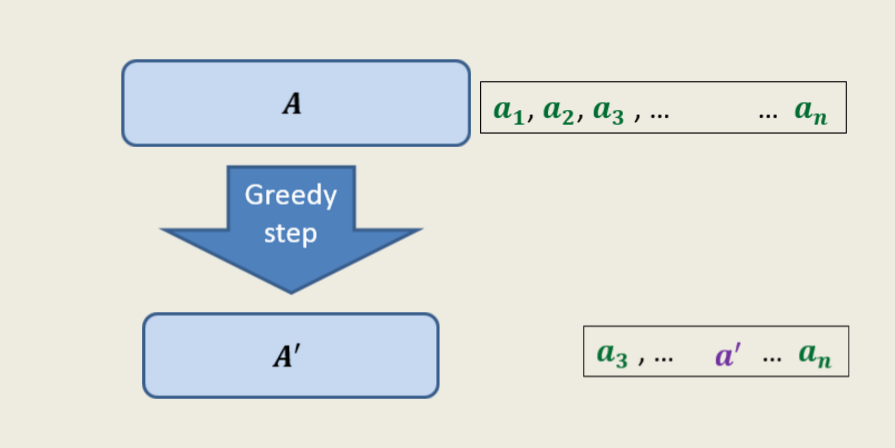
\includegraphics[width=0.5\columnwidth]{greedy1.png}
\caption{Greedy Step, where A represents BST B (Taken from Course Lecture Slides)}
\label{fig:one}
\end{center}
\end{figure}

Consider the following relation between $a_1,a_2 $ and $a^{'}$.

$$h(a^{'})= min(dist(a_{1},a_{2}))$$

The adjacency list of $a^{'}$ has vertices whose distance is minimum of distance from $a_1$ and distance from $a_2$. 

\textbf{Theorem:}
$$SUM(B) = SUM(B') + h_1 + h_2- w(v_1,v_2)$$
where SUM(B) is sum of h values of root of each corresponding tree for all vertices in B \\
$h_1, h_2 $ are the h values of the root of corresponding tree for the combining vertices \\
$w(v_1,v_2)$ is the minimum edge weight between all the vertices in the combining vertices/trees\\

\textbf{B' to B }
$$ SUM(B) \leq SUM(B') + h_1+ h_2 - w(v_1,v_2)$$

Since, when we break B' into $h_1$ and $h_2$, we get B. So, this is the maximum possible value that SUM(B) can achieve, by construction.

\textbf{B to B' }
$$ SUM(B') \leq SUM(B) - h_1- h_2 + w(v_1,v_2)$$

because the weight, w($v_1,v_2$) is the maximum that we can get after moving from B to B'.\\

From above two statements, we can conclude that :

$$SUM(B) = SUM(B') + h_1 + h_2- w(v_1,v_2)$$

\subsection{Proof of Correctness}
\textbf{$T^*$ is consistent with G: }\\
Simply by construction of tree, we can see that h value of LCA is less than or equal to dist($v_i$ , $v_j$), since while combining two trees, we are always taking the minimum distance between the two trees.\\

Also, Since we are taking edges in increasing order of edge weight, so h(u) $\geq$ h(v), if u is parent of v.\\ \\
\textbf{For any other tree T' consistent with G, the following condition holds for each $v_i$ , $v_j$ :
\emph{“distance between $v_i$ and $v_j$ in T′ is less than or equal to their distance in $T^*$.”}}\\ 
This can be proved by using induction on size of tree. For Base Case, When we combine two trees with one vertex each. Clearly, the h value of the combined node or the LCA will be the distance between the two vertices. Also, this is the maximum possible value that h can take. \\

For Induction Step, Assume that all trees at any stage in S satisfy the above condition i.e. h values are maximal. Now, combining two trees ($t_1$, $t_2$), the h value of $t_{1,2}$ is the minimum distance between the $t_1$ and $t_2$. Now, consider the following two cases:\\
\emph{h($t_{1,2}$) is less than the above value: }In this case we can easily increase the h value.\\
\emph{h($t_{1,2}$) is greater than the above value: } Now, the tree will violate the condition of being consistent with G, since h of LCA has to be less than or equal to distance between any two vertices.\\

Thus we prove by contradiction that the above assigned h value is optimal.

\subsection{Pseudo-Code}
Consider the following psedo-code which has the fastest implementation of the above algorithm.
\begin{algorithm}
\caption{Hierarchical Metric}
\label{hm}
\begin{algorithmic}[1]
\Procedure{Hierarchical(G)}{}
\State Initialise S 
\State Add closest neighbor to the front in all adjacency lists \Comment{\parbox[t]{.2\linewidth}}{O($n^2$)} 
\State Construct BST B \Comment{\parbox[t]{.2\linewidth}}{O(nlog(n))} 
\While { $Size(B) > 1$ } \Comment{\parbox[t]{.2\linewidth}}{ n-1 iterations} 
\State ( $B^{'}$, $S^{'}$ ) $\gets$ Greedy Step (B, S) \Comment{\parbox[t]{.2\linewidth}}{O(n)} 
\EndWhile
\EndProcedure
\end{algorithmic}
\end{algorithm}

\subsection{Time Compexity}
\emph{Constructing B:} O($n^2$ + nlog(n))\\
\emph{Greedy Step:} O(n)\\
\emph{Total Iterations Required:} O(n)\\
\emph{Cost of while loop:} O($n^2$)\\
\emph{Total Time Complexity: } O($n^2$)

\subsection{Note}
\begin{itemize}
\item $T^*$ is not unique, since in this solution we are constructing a binary tree, but one can construct a non-binary tree if two edge weights are equal. However, the h values will be same in both cases.
\item This problem is similar to MST, and for constructing an MST, the best solution is of time O(m+ nlog(n)) using fibonacci heap. Since m is of O($n^2$), so the optimal solution in that case using MST will be also of O($n^2$).
\item Instead of maintaining BST B, we can also use a sorted array to have the same functionality and time complexity will remain same, since extracting and inserting already costs O(n).
\end{itemize}

\section{Problem 2}
\subsection{Intuition}
We have to keep $O(\sqrt{n})$ edges for each vertex on an average. Since, maximum number of edges allowed are $O(n^{3/2})$, we can have O(n) nuber of edges for O($\sqrt{n}$) number of vertices.

\subsection{Algorithm}
\subsubsection{Pseudo-Code}
\begin{algorithm}
\caption{An inspirational Algorithm}
\label{hm}
\begin{algorithmic}[1]
\State $E_S \gets \phi$
\While { size(E) $>$ 0 }  \Comment{\parbox[t]{.6\linewidth}}{ We can also stop when size(E) $<$ $n^{3/2}$ }
\State Pick any vertex v from G
\If {degree(v) $\leq \sqrt{n}$ }
\State Add all edges incident on v to $E_S$
\State Remove v and all edges incident on v from G
\Else
\State Remove one of the edges from v from all 4-length cycles containing v formed by edges to already covered vertices
\State Remove all direct internal edges between uncovered neighbors(3-length cycle) 
\State Add all edges incident on v to $E_s$ 
\State Mark v as covered
\State Remove v and all edges incident on v from G if the number of uncovered neighbors is less than $\sqrt{n}$
\State Mark the uncovered neighbors as covered if the number of uncovered edges is greater than $\sqrt{n}$
\EndIf
\EndWhile
\State return $E_s$
\end{algorithmic}
\end{algorithm}
\subsubsection{Description}

We are actually making groups of vertices of size greater than equal to $\sqrt{n}$. Every group has a pivot vertex which can also be a member of another group. But, other than pivot element, each vertex will either belong to a group or remain independent. \\

While making groups, we only take unvisited neighbors as a group member to satisfy the above condition.\\

If a vertex has multiple edges to a single group, then it will clearly form a cycle of length 4, so we keep only one of those edges. And after this, if the number of uncovered neighbors of that vertex is less than $\sqrt{n}$, then we remove that vertex and all its incident edges, since there are only $\sqrt{n}$ possible groups possible, so this vertex has less than $2\sqrt{n}$ edges. Otherwise, we will make this vertex a pivot and all its uncovered/ungrouped neighbors as covered/grouped.

\subsection{Proof of Correctness}
\subsubsection{Size($E_S$) is of O($n^{3/2})$}
\begin{itemize}
\item Every pivot vertex may have O(n) edges in $E_S$.There can be atmost $\sqrt{n}$ groups/pivots, since a group has more than $\sqrt{n}$ vertices and we have only n vertices ($\sqrt{n}*\sqrt{n} = n $).
\item At any stage if a vertex has degree less than $\sqrt{n}$, we are removing that vertex from G and it contributes only O($\sqrt{n}$) edges to $E_S$. And clearly , such vertices can not be greater than n.
\item Each non-pivot covered vertex v will have atmost one edge to any particular group(removed cycle of 4 from covered vertices), and we have already included all non-group edges from v in the previous case. So, for each such v we will count only O($\sqrt{n}$) edges. Clearly, there can be atmost n such vertices.
\end{itemize}
\textbf{No of edges from each case in $E_S$: }\\
\emph{From Pivot: } $O(\sqrt{n}) * O(n) = O(n^{3/2})$\\ 
\emph{From Non-Group Edges: }$ O(n) * O(\sqrt{n}) = O(n^{3/2})$\\ 
\emph{From Non-Pivot Group Edges: }$ O(n) * O(\sqrt{n}) = O(n^{3/2})$\\ 
\emph{Total Count: } $O(n^{3/2})$

\subsubsection{Consistency}
As mentioned in the problem statement, to achieve consistency, it suffices if for each edge (u,v) $\in$ E, (u,v) $\notin E_S$  , there exists a path of at most 3 edges in H connecting u and v. So, Consider the following four cases.

\begin{itemize}
\item \textbf{Both vertex in same group: }Clearly, there exists a path of length two passing through pivot of the group.
\item \textbf{Both vertex (u,v) in different groups: } There exists atleast one edge (u,x) where x $\in$ Group(v). Let the pivot of Group(v) be w. Then, the path of length 3 is (u,x,w,v).
\item \textbf{One vertex in a group: } A vertex is not in group only when its degree is less than $\sqrt{n}$, and in such cases we have included the edge.
\item \textbf{Both not in any group: }In such cases, either we have stored a direct edge or there exists a path of 2 passing through a non-pivot grouped vertex.
\end{itemize}
Thus, there exists a path of atmost 3 in $E_S$ between any two neighbors in G.

\subsubsection{Termination}
After formation of maximal groups,suppose we don't have any vertex v with degree(v) $\leq \sqrt{n}$. This is the only case when the algorithm gets stuck. We will not have any free vertex in such cases, we only have vertices in groups. Now, consider any non-pivot grouped vertex, since there at most $\sqrt{n}$ groups, so the this vertex will have at most $\sqrt{n}$ edges, thus its degree is less than or equal to $\sqrt{n}$.  Hence, by contradiction we show that there always will be a vertex with degree less than or equal to $\sqrt{n}$.

\subsection{Implementation}
We can use BFS(only traversing neighbor and next neighbor) to implement the algorithm in O(m+n) time. \\

\begin{itemize}
\item First, construct maximal groups in O(m+n) time. We can construct groups by iterating over the the neighbors of all vertices with degree greater than $\sqrt{n}$. After this step, we would have removed all the direct internal edges between non-pivot group members. In this process, for each vertex we are visiting their neighbors only once, so it will cost only O(m+n) time.  We also don't have any free vertices because we have deleted every vertex with degree less than or equal to $sqrt(n)$. Also, keep a label for each group.  
\item Second, To remove all 4-length cycles between groups, for each non-pivot vertex, just check all the neighbors and if more than one of the neighbors belong to the same group, keep only one of those edges. Since for each vertex, we are traversing it's neighbors only once, so total cost will be O(m+n).
\end{itemize} 
\end{document}


